\documentclass[11pt]{article}

\usepackage[margin=1in]{geometry}
\usepackage{amsmath}
\usepackage{booktabs}
\usepackage{longtable}
\usepackage{graphicx}
\usepackage[dvipsnames]{xcolor}
\usepackage{tikz}
\usetikzlibrary{arrows.meta, positioning}
\usepackage[colorlinks=true, linkcolor=MidnightBlue, citecolor=MidnightBlue, urlcolor=MidnightBlue]{hyperref}
\usepackage{natbib}
\usepackage{siunitx}

\title{TB Infectious Disease Modeling: Background and Literature Review}
\author{}
\date{}

\begin{document}
\maketitle

\section{TB epidemiology and natural history}
\label{sec:epi}

Tuberculosis (TB) is caused by \textit{Mycobacterium tuberculosis} and transmitted primarily via the airborne route. Transmission typically requires prolonged contact, and infectiousness varies by disease stage. The majority of infected individuals do not develop immediate symptomatic disease; instead they enter a latent state with an elevated risk of future progression \citep{vynnycky1997natural}. A commonly cited rule of thumb is that roughly 5--10\% of infected individuals progress to active disease within the first few years, with a smaller but persistent risk of reactivation thereafter \citep{vynnycky1997natural, who2025global}.

Global burden remains substantial. The WHO Global Tuberculosis Report 2025 documents ongoing high incidence in multiple regions and highlights the role of HIV co-infection in disease progression and mortality \citep{who2025global}. The latent TB reservoir is large: a recent re-estimation suggests roughly one quarter of the global population has latent infection \citep{houben2016latent}.

\subsection{Current global burden and regional distribution}

In 2024, an estimated 10.7 million people fell ill with TB worldwide, equivalent to 131 new cases per 100{,}000 population \citep{who2025global}. Eight countries accounted for two-thirds of global cases: India (25\%), Indonesia (10\%), the Philippines (6.8\%), China (6.5\%), Pakistan (6.3\%), Nigeria (4.8\%), Democratic Republic of the Congo (3.9\%), and Bangladesh (3.6\%).

Table~\ref{tab:who_region_2024} shows the most recent cross-sectional estimates by WHO region. The South-East Asia Region (SEAR) and the African Region carry the highest absolute and per-capita burden, respectively, while the European and Americas regions have much lower rates.

\begin{table}[h]
\centering
\caption{Estimated TB incidence by WHO region, 2024. Source: WHO Global Tuberculosis Report 2025 \citep{who2025global}. Note: Indonesia was reclassified from SEAR to WPR by WHA Resolution 78 (2025), affecting comparability with earlier editions.}
\label{tab:who_region_2024}
\begin{tabular}{lrr}
\toprule
\textbf{WHO Region} & \textbf{New cases (thousands)} & \textbf{Rate per 100{,}000} \\
\midrule
South-East Asia    & 3{,}680 & 201 \\
Western Pacific    & 2{,}910 & 131 \\
Africa             & 2{,}620 & 207 \\
Eastern Mediterranean & 920  & 112 \\
Americas           &   350  &  33 \\
Europe             &   204  &  22 \\
\midrule
\textbf{Global}    & \textbf{10{,}700} & \textbf{131} \\
\bottomrule
\end{tabular}
\end{table}

\subsection{Twenty-year trend in global incidence}

Global TB incidence has been declining since approximately 2000, driven by improved treatment coverage, HIV antiretroviral therapy (ART) scale-up in high-burden African countries, and economic development. The WHO End TB Strategy, adopted in 2015, set a baseline rate of approximately 142 cases per 100{,}000 and targets a 50\% reduction by 2025 and a 90\% reduction by 2035.

Table~\ref{tab:global_trend} presents global TB incidence at approximately five-year intervals from 2005 to 2024. Values for 2005--2012 are approximate estimates from the WHO Global Tuberculosis Control Reports published in those years; more recent values are from the 2021 and 2025 editions. All estimates carry considerable uncertainty and historical series are revised retrospectively as new national prevalence survey data become available; absolute case counts before 2015 are particularly subject to upward revision and are not reported here.

\begin{table}[h]
\centering
\caption{Global TB incidence rate, selected years 2005--2024. Values marked $\approx$ are approximate or derived from earlier report editions. Source: WHO Global Tuberculosis Reports, various years \citep{who2025global}.}
\label{tab:global_trend}
\begin{tabular}{lcc}
\toprule
\textbf{Year} & \textbf{Rate per 100{,}000} & \textbf{New cases (millions)} \\
\midrule
2005  & $\approx$179 & --- \\
2010  & $\approx$160 & --- \\
2015  & $\approx$142 & $\approx$10.4 \\
2019  & $\approx$130 & $\approx$10.0 \\
2020  & 127          & 9.9  \\
2022  & $\approx$133 & $\approx$10.6 \\
2024  & 131          & 10.7 \\
\bottomrule
\end{tabular}
\end{table}

The COVID-19 pandemic disrupted TB services sharply in 2020, when newly diagnosed cases fell from 7.1 million in 2019 to 5.8 million in 2020. This reduction in detection is estimated to have increased the pool of undiagnosed, untreated cases and driven a 4.6\% rise in estimated incidence between 2020 and 2023 (reaching 10.8 million new cases in 2023, the highest estimate in the modern era). By 2024, improved case-finding had reversed this trend, with incidence falling back to 131 per 100{,}000 for the first time since the pandemic \citep{who2025global}.

Regional trends diverge substantially. Between 2015 and 2024, the European Region achieved the largest proportional reduction (39\%), driven primarily by the Russian Federation. The African Region declined 28\%, reflecting ART scale-up. Progress was slower in the South-East Asia Region (16\%) and the Eastern Mediterranean Region (5.9\%). In contrast, the Western Pacific Region and the Americas showed small \textit{increases} of 1.7\% and 13\% respectively over the same period, the latter driven by sustained upward trends in Brazil and several neighbouring countries.

TB prevalence (active disease at a point in time) exceeds incidence because cases persist for months to years before treatment or self-resolution. WHO estimates global TB prevalence as roughly 1.5--2$\times$ the incidence count, implying approximately 15--20 million people living with active TB globally in recent years; however, precise prevalence figures by region require periodic national prevalence surveys and carry wider uncertainty intervals than incidence estimates. Country-level prevalence estimates are published in the WHO Global Tuberculosis Report app and country profiles.

\subsection{Natural history in the absence of treatment}
Natural history in the absence of treatment is prolonged. A systematic review of pre-chemotherapy era data estimates untreated pulmonary TB has an average duration of about three years and high case fatality, especially in smear-positive disease \citep{tiemersma2011natural}. These estimates provide important anchors for model parameters related to infectious duration and TB-specific mortality.

Recent evidence emphasizes a spectrum of TB disease states, including minimal disease (non-infectious), subclinical disease (infectious but asymptomatic), and clinical disease (symptomatic and infectious) \citep{richards2023spectrum}. Subclinical TB has epidemiological relevance because it contributes to transmission while escaping symptom-based detection \citep{kendall2021subclinical}.

\begin{figure}[h]
\centering
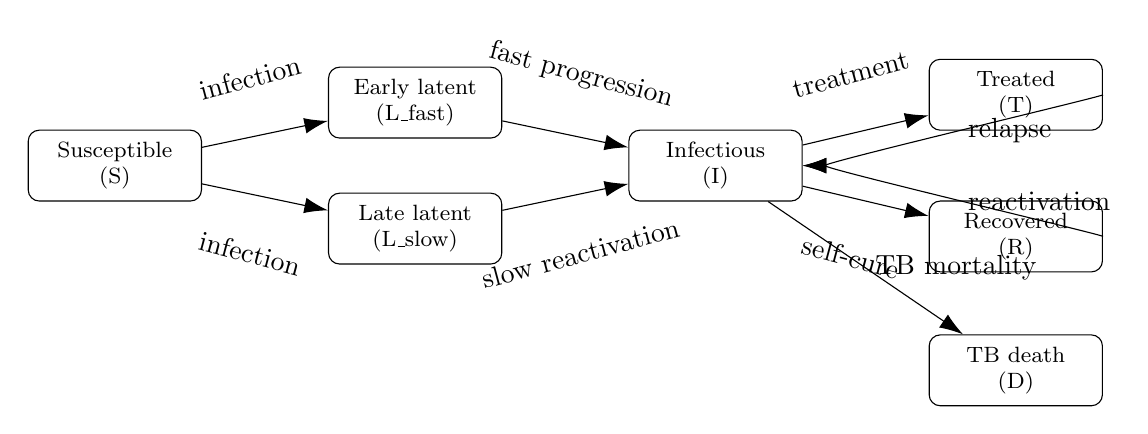
\begin{tikzpicture}[
  node distance = 1.6cm,
  box/.style = {draw, rounded corners, align=center, minimum width=2.2cm, minimum height=0.9cm, font=\footnotesize},
  arrow/.style = {-{Latex[length=3mm,width=2mm]}}
]
\node[box] (S) {Susceptible\\(S)};
\node[box, right=of S, yshift=0.8cm] (Lf) {Early latent\\(L\_fast)};
\node[box, right=of S, yshift=-0.8cm] (Ls) {Late latent\\(L\_slow)};
\node[box, right=of Lf, yshift=-0.8cm] (I) {Infectious\\(I)};
\node[box, right=of I, yshift=0.9cm] (T) {Treated\\(T)};
\node[box, right=of I, yshift=-0.9cm] (R) {Recovered\\(R)};
\node[box, right=of I, yshift=-2.6cm] (D) {TB death\\(D)};

\draw[arrow] (S) -- node[above, rotate=15, outer sep=0.5cm] {infection} (Lf);
\draw[arrow] (S) -- node[below, rotate=-15, outer sep=0.5cm] {infection} (Ls);
\draw[arrow] (Lf) -- node[above, rotate=-15, outer sep=0.5cm] {fast progression} (I);
\draw[arrow] (Ls) -- node[below, rotate=15, outer sep=0.5cm] {slow reactivation} (I);
\draw[arrow] (I) -- node[above, rotate=15, outer sep=0.5cm] {treatment} (T);
\draw[arrow] (I) -- node[below, rotate=-15, outer sep=0.5cm] {self-cure} (R);
\draw[arrow] (I) -- node[right] {TB mortality} (D);
\draw[arrow] (T) .. controls +(right:1.2cm) and +(right:1.2cm) .. node[right] {relapse} (I);
\draw[arrow] (R) .. controls +(right:1.2cm) and +(right:1.2cm) .. node[right] {reactivation} (I);
\end{tikzpicture}
\caption{Simplified TB natural history used for the toy model.}
\label{fig:tb_flow}
\end{figure}

\section{Mathematical modeling approaches for TB}

Compartmental ordinary differential equation (ODE) models are a standard entry point for infectious disease modeling. For TB, simple SIR or SEIR models are often insufficient because latency can last years, progression is heterogeneous, and treatment modifies infectious duration. As a result, TB models commonly split the latent period into fast and slow progressors, include explicit treatment compartments, and allow for reactivation and relapse \citep{vynnycky1997natural}.

Key mathematical tools include the computation of the basic reproduction number $R_0$ using the next-generation matrix method \citep{diekmann1990r0}. Parameter estimation methods range from least squares to Bayesian inference, and sensitivity analyses (one-at-a-time, PRCC, or tornado plots) are used to identify dominant drivers of transmission dynamics.

Deterministic ODE models provide transparent, interpretable baselines and are well suited for learning. Stochastic or agent-based approaches become more relevant when heterogeneity, household structure, or small population effects dominate the dynamics. This project starts with a deterministic ODE model and provides a clear path toward extensions.

\subsection{Stochastic ODE models and uncertainty analysis}

Deterministic ODE models suppress variability and mask uncertainty in parameter estimates. \citet{blower1995dynamics} developed a stochastic framework for TB that couples the ODE system with Monte Carlo sampling over uncertain parameters to produce probabilistic projections of epidemic trajectories. A key finding is that TB epidemics evolve over decades to centuries---a timescale set by the slow progression of latent infection and the density of the susceptible pool---so short-horizon projections may be misleading without propagating uncertainty from input parameters. Sensitivity analysis methods such as partial rank correlation coefficients (PRCC) are used to identify which parameters most drive uncertainty in $R_0$ and incidence projections. This approach remains useful as a complement to deterministic baselines when communicating uncertainty to policy audiences.

\subsection{Extended compartmental models with drug resistance and reinfection}

More complex ODE models stratify the population further to capture phenomena absent from simple SEIR-like structures. \citet{trauer2014construction} constructed a ten-compartment deterministic model calibrated to high-burden settings in the Asia-Pacific. The model adds: (i) a declining hazard of active disease with time since infection, (ii) explicit reinfection during latency and after treatment, (iii) a separate multidrug-resistant (MDR-TB) strain with fitness costs and de novo resistance during treatment, and (iv) a vaccine compartment with temporary efficacy. A critical finding is that the model could not reproduce observed incidence trajectories without allowing reinfection during latency, indicating this mechanism is epidemiologically important in high-burden settings. Additionally, even a modestly fit MDR-TB strain becomes dominant at equilibrium under most parameterizations, illustrating how treatment coverage interacts with drug resistance dynamics in ways that simple two-strain ODE models capture efficiently.

\subsection{Individual-based and microsimulation models}

When population heterogeneity is a first-order concern---for example, when modeling targeted interventions in low-incidence settings---individual-based or microsimulation models offer advantages that ODE compartmental models cannot easily replicate. \citet{goodell2019california} developed a discrete-time stochastic microsimulation for California in which each simulated individual carries attributes including age, race/ethnicity, nativity, and medical risk factors (HIV, diabetes, immunosuppressive therapy, among others) that modify their reactivation rate. The model captures semi-random mixing by nativity group and is calibrated to historical case counts from 2001 to 2014. Compared to population-level ODE projections, the individual-based structure allows the authors to estimate cost per QALY for interventions targeted at specific risk groups, and to model the threshold scale-up needed to hit the WHO pre-elimination target of $<10$ cases per million. The trade-off is substantially higher computational cost and greater data requirements for demographic parameterization.

\subsection{Risk-factor stratified models: nutrition and biomarkers}

A second class of model extensions stratifies the population along a continuous biological risk factor---most commonly body mass index (BMI) or glycaemic status---rather than by transmission or drug-resistance status. The key modelling step is to replace scalar progression and treatment-outcome rates with values that depend on the stratum, allowing the force of infection on downstream compartments to vary by nutritional or metabolic state.

\paragraph{Nutrition and BMI.}
\citet{oxlade2015undernutrition} constructed a compartmental transmission model for the Central Eastern states of India in which the population is stratified by BMI. Progression rates from latent to active TB are assigned per stratum following empirical estimates of the BMI--TB risk relationship, and strata exchange members as nutritional status changes over time. Simulations showed that even a modest reduction in undernutrition could avert 4.8 million TB cases and 1.6 million TB deaths over 20 years; complete elimination of undernutrition was projected to avert 9.4 million cases, underscoring how deeply TB burden in high-burden settings is driven by nutritional risk. Building on this framework, \citet{mandal2024undernutrition} applied a comparable deterministic compartmental model to the WHO South-East Asia Region, explicitly stratifying individuals as well-nourished or undernourished and coupling the model to country-specific undernutrition prevalence estimates. The study simulated two intervention types---nutritional rehabilitation of TB patient contacts versus a population-wide programme---and found that the population-wide approach reduces cumulative incidence 2--3 fold more than the targeted contact strategy; in India specifically, rehabilitating 30\% of the undernourished population annually would avert 15.9\% of cumulative TB incidence between 2023 and 2030.

A more recent extension couples the TB transmission model to an external food-system model \citep{clark2025nutritional}. The TB component uses four explicit BMI strata (moderate--severe thinness, mild thinness, normal, overweight), with stratum-specific progression and treatment-outcome rates. The LandSyMM food-system model projects how supply-chain shocks---parameterised as the stylised energy-price and export-restriction scenarios arising from the war in Ukraine---shift the population-level BMI distribution, which is then fed forward into the TB model. In a worst-case scenario, the combined shock increases TB incidence by 5.0\% and mortality by 4.9\% in India by 2035, equivalent to an additional 1.1 million TB episodes. The approach illustrates how global macroeconomic shocks can propagate through nutritional pathways into infectious disease burden, and provides a template for coupling TB models to broader health determinant models.

\paragraph{Diabetes as a biomarker-mediated risk factor.}
Diabetes mellitus (DM) substantially increases the risk of TB and is increasingly prevalent in high-burden settings. \citet{awad2019diabetes} developed an ODE model stratified by DM status, calibrated to India, and used it to map ten plausible biological pathways by which DM modifies TB natural history and treatment outcomes---including increased susceptibility, accelerated fast progression, higher smear-positivity, elevated infectiousness (through higher bacterial load), increased TB mortality, and reduced treatment success. Using a standardised effect size for each pathway, the model quantifies both direct effects (captured by hazard ratios comparing DM to non-DM individuals) and indirect effects arising from onward transmission through the expanded infectious pool. A notable finding is that pathways that have no impact on the individual-level hazard ratio, such as increased infectiousness, can still account for up to 30\% of the population-attributable fraction through amplified transmission---a result inaccessible to conventional epidemiological designs. This work demonstrates that biomarker-stratified ODE models can reveal mechanistic contributions to population-level TB burden that observational hazard-ratio analyses systematically miss.

Collectively, these risk-factor stratified models share a structural logic: the standard compartmental states ($S, L, I, T, R$) are replicated across risk strata, stratum-specific rates substitute for scalar parameters, and movement between strata represents changes in the underlying biomarker. The design choice of how many strata to use, and how to parameterise inter-stratum transition rates from survey data, is a key modelling decision with direct implications for policy inference.

\section{Economic evaluation approaches for TB}

Economic evaluation methods are used in TB research to assess whether interventions deliver sufficient health benefit relative to their costs, and to prioritize limited resources across competing strategies. The three most common frameworks are cost-effectiveness analysis (CEA), cost-utility analysis (CUA), and budget impact analysis (BIA). CEA and CUA typically compute an incremental cost-effectiveness ratio (ICER):
\[
  \text{ICER} = \frac{\Delta \text{Cost}}{\Delta \text{Health outcome}},
\]
where the health outcome is expressed in natural units (e.g., cases averted, deaths averted) for CEA, or in quality-adjusted life years (QALYs) or disability-adjusted life years (DALYs) for CUA. The WHO convention expresses TB burden in DALYs, making cost-per-DALY-averted the dominant metric in TB intervention evaluations. An intervention is conventionally deemed cost-effective if its ICER falls below one to three times the per-capita GDP of the country under study, though this threshold is contested.

A distinctive feature of TB economic evaluations is that they frequently integrate the economic analysis directly with a transmission model. Because TB interventions such as improved diagnostics or treatment completion reduce transmission, a static model that ignores downstream prevented infections will underestimate the benefit. \citet{menzies2012xpert} demonstrate this approach: they coupled a calibrated dynamic transmission model for five southern African countries with a cost module to evaluate Xpert MTB/RIF versus sputum-smear diagnosis. Over a ten-year horizon, the intervention was projected to avert 132{,}000 TB cases and 182{,}000 deaths at a cost-effectiveness of approximately \$959 per DALY averted---within the cost-effectiveness threshold for most of the study countries. Importantly, a large fraction of the additional costs arose from antiretroviral therapy for HIV-positive individuals who survived due to better TB case-finding, illustrating how transmission-model-based economic evaluations can reveal unexpected cost drivers through downstream effects.

Budget impact analysis differs from CEA in that it asks not whether an intervention is worth its cost, but whether the health system can afford it. For TB, scale-up of MDR-TB treatment or novel diagnostics often passes cost-effectiveness thresholds yet fails budget impact analyses because the upfront financial requirement exceeds available program budgets. Taken together, CEA/CUA and BIA serve complementary roles: the former informs whether to adopt an intervention, and the latter informs whether and how quickly the health system can realistically do so.

\section{The SELT(R) model used in this project}

The toy model implemented here is a deterministic compartmental ODE model with six state variables, chosen to reflect the biological features described in Section~\ref{sec:epi}: the two-speed nature of latency, the possibility of self-cure, the modification of infectious duration by treatment, and excess TB-specific mortality.

\subsection{Compartments and biological rationale}

\begin{itemize}
  \item \textbf{Susceptible ($S$)} -- individuals with no prior infection, fully at risk.
  \item \textbf{Early latent ($L_\text{fast}$)} -- recently infected fast progressors ($\sim$10\% of new infections), who develop active TB within months.
  \item \textbf{Late latent ($L_\text{slow}$)} -- recently infected slow progressors ($\sim$90\%), who carry a low but persistent long-term reactivation risk.
  \item \textbf{Infectious ($I$)} -- active pulmonary TB; symptomatic or subclinical, capable of transmission.
  \item \textbf{Treated ($T$)} -- individuals on treatment; no longer contributing to transmission, but subject to relapse.
  \item \textbf{Recovered ($R$)} -- self-cured; no longer infectious, but reactivation is possible.
\end{itemize}

The flow diagram (Figure~\ref{fig:tb_flow}) summarizes all transitions. The full ODE system, $R_0$ expression, and default parameter values with literature sources are documented in notebook \texttt{01\_tb\_model.ipynb}.

\bibliographystyle{plainnat}
\bibliography{references}

\end{document}
